\subsection{Caso testigo}
\label{caso-testigo}

Habiendo desarrollado la propuesta de rediseño que motiva el presente trabajo, creemos conveniente tomar un caso testigo que sirva de ejemplo práctico para hacer concretos los conceptos teóricos que hemos tenido en cuenta para el análisis, a la vez que sirva de disparador para una implementación preliminar acotada del nuevo diseño sobre los elementos de la nube de servicios. De aquí en más, para distinguir la nube actual (el Integrador) de la nueva arquitectura que estamos planteando, utilizaremos el nombre clave \cloud para hacer referencia a esta última.

\subsubsection{Alcance}

La situación que utilizaremos como caso testigo es el proceso de registro de un nuevo usuario de \gls{acro:sso} de la nube de servicios de la \unlp. Si bien \textit{a priori} puede parecer un tanto sencillo para tomarlo de referencia, una vez que definamos en concreto todos los pasos involucrados en este proceso se hará evidente la elección realizada.

Aquellos agentes que forman parte del personal de la UNLP pueden tener un usuario único para acceder a las aplicaciones que nuestra Dirección desarrolla, ya sea para consultar sus recibos de haberes, utilizar una aplicación como parte de sus tareas diarias, presentar proyectos de extensión cuando la convocatoria se encuentre abierta o para acceder a cualquier aplicación que a futuro pudiéramos publicar. Para registrar su usuario, el agente dispone de dos vías:

\begin{itemize}
  \item La vía analógica: solicitando la creación del usuario, de manera presencial y por escrito, a la oficina de Personal de alguna de las Dependencias donde desempeña sus funciones. Por tratarse de un proceso manual y \eng{offline}, no lo consideraremos para este caso testigo.

  \item La vía digital: utilizando la \hyperref[anexo:detalle-clientes:sso]{aplicación de autogestión} que hemos desarrollado para realizar el registro del nuevo usuario en línea. \textit{Esta} es la vía que utilizaremos en nuestro planteo.
\end{itemize}

En el proceso de autogestión de un nuevo usuario, el agente debe completar los datos solicitados en una serie de pasos preestablecidos que lo guían hasta llegar a obtener el acceso a las aplicaciones que utilizan este esquema de \gls{acro:sso}\footnote{En realidad, inicialmente obtiene acceso únicamente a ver sus \hyperref[anexo:detalle-clientes:recibos]{recibos de haberes} y cargar su \textit{currículum de extensionista} en la aplicación de \hyperref[anexo:detalle-clientes:extension]{Proyectos de Extensión}. Para ingresar al resto de las aplicaciones un usuario autorizado le debe asignar los roles necesarios para cada aplicación.}. Podemos resumir estos pasos para el registro en:

\begin{enumerate}
  \item El agente ingresa a la aplicación de autogestión e indica que desea registrar un nuevo usuario. Para esto, debe ingresar una dirección de correo institucional propia para recibir por esa vía un vínculo de acceso para comenzar efectivamente el registro de su nuevo usuario.

  \item Al ingresar al vínculo de acceso que le llega a su correo, la aplicación solicita al agente que se identifique mediante su tipo y número de documento de identidad y en respuesta a ésto le indica si se lo tiene entre los agentes de la Universidad que aún no tienen usuario de acceso único.

  \item Una vez identificado el agente, se le sugiere un nombre de usuario siguiendo el formato estándar de nombres de usuario, el cual puede ser modificado como parte de la carga de información que se está realizando. Se chequea que este usuario no se encuentre en uso y que respete dicho formato estándar.

  \item Luego de elegido el nombre de usuario, se permite al agente ingresar una dirección de correo electrónico alternativa para tener un segundo medio de contacto.

  \item Para cerrar la carga de datos personales, se le pide que indique en qué Dependencias de la UNLP presta servicios. Esto se hace a modo de \gls{term:captcha} para evitar \eng{bots} que intenten registrar usuarios en masa y personas malintencionadas que deseen registrar usuarios en nombre de agentes reales.

  \item Al validar correctamente esta información, se le presentan todos los datos ingresados para su confirmación y si el agente los acepta, se le envía un correo electrónico con un formulario para presentar firmado en la oficina de Personal de alguna de las Dependencias donde presta servicios, teniendo un paso de validación humana de la información\footnote{Este paso adicional, si bien puede sonar contradictorio con el resto del proceso \eng{online} planteado, fue requerido por las autoridades de la Universidad para fortalecer los chequeos realizados sobre los datos recibidos mediante este servicio público de registro.}.

  \item Luego de presentar ese formulario y que sus datos sean debidamente corroborados por algún empleado de la oficina de Personal correspondiente, el usuario es aprobado y se dispara el envío de un nuevo correo al agente, en el cual se le consignan su usuario y una clave provisoria para que ingrese por primera vez a los sistemas de la UNLP. Con este paso, se finaliza el proceso de registro del nuevo usuario para el agente.
\end{enumerate}

Desde el punto de vista de nuestra aplicación, este proceso se ve un tanto reducido ya que no es necesario que incluyamos los pasos que ocurren por fuera del \textit{mundo virtual} o en la aplicación de gestión que utilizan los empleados de las oficinas de Personal de las Dependencias, ya que quedan afuera de su alcance. Formalizaremos los pasos que se realizan en este sistema con el diagrama de flujos presentado a continuación para su mayor referencia.

\begin{figure}[H]
  \centering
  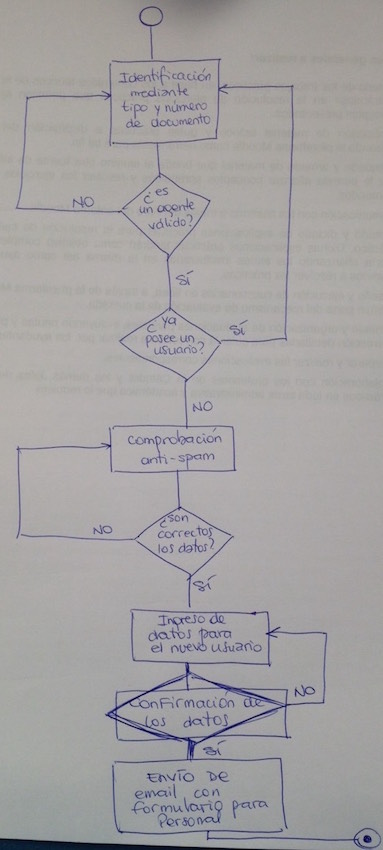
\includegraphics[width=\textwidth,height=0.5\textheight,keepaspectratio]{src/images/05-capitulo-5/diagrama-flujo-registro.jpg}
  \caption{Proceso de autoregistro de un nuevo usuario de acceso único}
  \label{fig:diagrama-flujo-registro}
\end{figure}

Realizando una descomposición en servicios del proceso anterior, identificamos las siguientes dependencias con servicios de la \cloud:

\begin{itemize}
  \item \textbf{Servicios de referencia:} para visualizar y marcar las Dependencias (o Unidades Académicas) y para ofrecer para su selección los tipos de documento de identidad.

  \item \textbf{Servicios de información sobre el personal:} como vía para identificar a la persona y luego consultar las Unidades Académicas en las cuales presta sus servicios.

  \item \textbf{Servicios de usuarios:} para la consulta de la existencia de un usuario para la persona seleccionada, sugerir nombres de usuario que respeten el formato estándar definido y para la creación del nuevo usuario.

  \item \textbf{Servicio de notificaciones:} para el envío de correos electrónicos. Destacamos en este punto que para limitar el alcance del caso testigo dejaremos la implementación de este servicio como un trabajo a futuro, ya que su existencia no es limitante para poder desarrollar los pasos de registro que se realizan en línea.
\end{itemize}

El desarrollo del prototipo funcional implica:

\begin{itemize}
  \item Implementar desde cero los servicios de la \cloud antes mencionados (de referencia, de información sobre el personal y de usuarios), en los cuales incluiremos únicamente los \eng{endpoints} necesarios para solventar la lógica del caso testigo.

  \item Implementar desde cero una nueva versión de la aplicación cliente de registro, respetando los pasos antes descriptos, que consuma toda la información de los servicios de la \cloud. Esta nueva versión difiere en su concepción de la versión actualmente implementada en que no tendrá acceso a la base de datos de usuarios. De hecho, no tendrá acceso a \textit{ninguna} base de datos, ya que realizará todas sus operaciones de manera volátil dependiendo completamente de los servicios de la \cloud para acceder a la capa de persistencia en base de datos.

  \item Desarrollar una \textit{gema} (nombre que reciben las librerías reutilizables en el lenguaje Ruby) que encapsule la lógica de acceso a los servicios, desde la autenticación hasta la consulta y abstracción en objetos de las respuestas de sus \glspl{acro:api}, basándose en el estándar elegido para la codificación de la información.
\end{itemize}

Hemos elegido este caso testigo porque se compone de una serie de interacciones entre distintos servicios que brindan una noción de la complejidad que pueden tener las operaciones a realizar utilizando la nube de servicios, más allá de las simples consultas de datos de referencia que habitualmente manejamos. El hecho de incorporar diferentes servicios, englobados en distintas áreas de acción, nos permite también mostrar cómo funcionan las instancias de las aplicaciones que proveen esos servicios, cómo interactúan con la aplicación cliente y con los elementos intermediarios de la comunicación (entiéndase \eng{caches} compartidas, balanceadores de carga, \eng{proxies} reversos y la capa de mediación ofrecida por \nameref{soa:tecnologias:tyk}).

En este informe intentaremos no entrar en detalles innecesarios sobre la implementación de la aplicación cliente ni de la capa de lógica del negocio de los servicios, para sí ahondar sobre temas relevantes desde el punto de vista de la comprensión de las entidades participantes en las comunicaciones. Para su referencia, se adjunta al presente informe el código fuente de los distintos apartados que hemos implementado en este capítulo.


\subsubsection{Arquitectura}

Partiendo de lo propuesto en la \autoref{propuesta}, el primer paso dentro de la implementación del prototipo funcional para este caso testigo es acotar la arquitectura, diseñarla y preparar los nodos en ella involucrados. Para esto, pueden observarse en la \autoref{fig:arquitectura-caso-testigo} los componentes lógicos del prototipo:

\begin{itemize}
  \item \textbf{Aplicación de registro:} esta es la implementación de una aplicación cliente de la \cloud. Es la cara visible hacia los usuarios públicos, y si bien en este caso particular hemos decidido implementarla utilizando \gls{fw:rails} por cuestiones prácticas, podría implementarse utilizando otras tecnologías como \eng{frameworks} web JavaScript que se ejecuten meramente del lado del cliente, PHP o Java, por nombrar algunas. De todos los componentes de la arquitectura, este es el único que se encuentra lógicamente por fuera de la \cloud. Esta separación del resto la hacemos evidente porque en este caso se trata de una aplicación desarrollada por nosotros mismos, pero en el futuro bien podría tratarse de una aplicación desarrollada por terceros, pertenecientes o no a la \unlp.

  \item \textbf{API Gateway (ESB):} este nodo se encarga de ser la capa que aisla los clientes de la \gls{acro:api}, brindando el acceso a los mismos desde un único punto. Como hemos visto con anterioridad, es el encargado de autorizar las peticiones entrantes, chequear que se encuentren dentro de los límites para ellas establecidos, mantener y utilizar una capa de caching intermedio, y finalmente balancear la carga de los backends de servicios con un mecanismo de Round Robin que asigna una petición entrante \textit{no cacheada} a cada backend por vez. Complementariamente a esta tarea, el producto elegido en nuestro análisis para este rol (\nameref{soa:tecnologias:tyk}) provee una interfaz web de gestión para los usuarios internos que administran el acceso a los servicios (en principio, nosotros) con gráficos estadísticos del uso de nuestras \glspl{acro:api} que resulta de gran utilidad.

  \item \textbf{API de referencia:} esta, como el resto de las \glspl{acro:api} implementadas, provee un conjunto de servicios relacionados a una única incumbencia lógica, siguiendo el principio de una sola responsabilidad\footnote{También conocido como \eng{Single Responsibility Principle} en inglés. Este es uno de los cinco principios SOLID de diseño de software que apuntan a mejorar la calidad y facilidad de mantener de un desarrollo.} e implementando el \hyperref[microservicios]{patrón de microservicios} tratado con anterioridad. En el caso de este \eng{service component}, su incumbencia es brindar los servicios de consulta de datos de referencia acotados a los necesarios para alcance de este caso testigo: tipos de documento y unidades acdémicas. Se encuentra implementada con el framework \nameref{soa:tecnologias:rails} en su versión 5 en modo \texttt{--api}.

  \item \textbf{API de personal:} este nodo es otro \eng{service component} que se encarga de brindar los servicios relacionados a la información de personal de la \unlp. Esta es otra aplicación Rails versión 5 en modo \texttt{--api}.

  \item \textbf{API de usuarios:} otro \eng{service component} orientado a brindar acceso a las operaciones a realizar sobre los usuarios del esquema \gls{acro:sso}: gestión de usuarios y políticas de nombres de usuario. Al igual que en las \glspl{acro:api} anteriores, es una aplicación Rails 5 en modo \texttt{--api}.

  \item \textbf{API de notificaciones:} nodo que se dedica a la emisión de notificaciones (principalmente vía correo electrónico) que las aplicaciones cliente pudieran necesitar enviar. Es el \eng{service component} que en una aplicación monolítica sería reemplazado por el \eng{mailer} y el motor de generación de correos electrónicos. Similarmente a los casos anteriores, esta es otra aplicación Rails 5 en modo \texttt{--api}.

  \item \textbf{Capa de persistencia:} esta unidad de la arquitectura planteada es la encargada estrictamente del almacenamiento persistente de la información. Se trata de una base de datos MySQL, que pudiera estar replicada utilizando un modelo maestro-esclavo para conseguir redundancia y escalabilidad en el eje \textit{X}.

  \item \textbf{Cache compartida:} este componente de la arquitectura, de carácter opcional, beneficia en términos de escalabilidad y reducción de costos de procesamiento. Está implementado con un servidor de la base de datos clave-valor \gls{db:memcached}, que se utiliza como cache compartida entre las diferentes instancias de los \eng{service components} antes mencionados. Su principal función es evitar volver a calcular las respuestas que cualquiera de los servicios debiera brindar si antes ya se la generó (ya sea en la misma instancia del servicio u otra distinta) y los datos originales no han cambiado.
\end{itemize}

Para demostrar las posibilidades de escalabilidad de esta arquitectura, hemos replicado los nodos de servicios para correr dos instancias de cada uno, las cuales serán balanceadas de manera transparente por \nameref{soa:tecnologias:tyk}.

\begin{figure}
  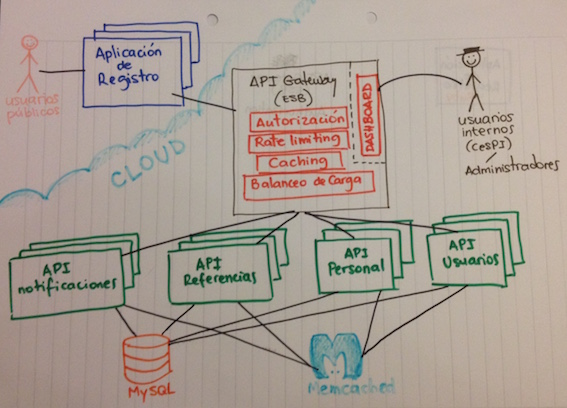
\includegraphics[width=\linewidth]{src/images/05-capitulo-5/arquitectura-caso-testigo.jpg}
  \caption{Visión lógica de la arquitectura del caso testigo}
  \label{fig:arquitectura-caso-testigo}
\end{figure}

\subsubsection{Desarrollo del prototipo funcional}

Para el desarrollo de la arquitectura de nuestro caso testigo hemos seguido los principios que utilizamos en nuestra oficina de trabajo, tanto en la metodología ágil de desarrollo empleada, como en las herramientas fundamentales que se basan en productos \eng{Open Source}:

\begin{itemize}
  \item Para el versionado de nuestro código utilizamos el sistema de control de versiones \gls{scm:git}, con la interfaz web que brinda el producto GitLab\footnote{\url{https://about.gitlab.com}}.

  \item Para el desarrollo usamos ambientes locales en nuestras computadoras, replicando un entorno similar a aquel en que finalmente vivirán las aplicaciones en producción.

  \item Para armar la topología de producción, utilizamos máquinas virtuales sobre un entorno de virtualización basado en Proxmox\footnote{\url{http://www.proxmox.com/en/proxmox-ve}}, en el cual creamos libremente tantas instancias virtuales como necesitamos.

  \item Para el sistema base de cada instancia virtual utilizamos una versión reducida de la distribución de GNU/Linux Ubuntu, que se encuentra modificada y simplificada para correr en máquinas virtuales consumiendo menos recursos.

  \item Para la resolución de los nombres de las instancias virtuales instalamos un servidor de DNS BIND9\footnote{\url{https://kb.isc.org/article/AA-01031}} utilizando el subdominios para cada host pertenecientes a la zona \url{tesis.desarrollo.unlp.edu.ar}.

  \item Para aislar la arquitectura y evitar problemas de seguridad, utilizamos un esquema de red privada local al servidor de Proxmox, al cual accedimos mediante modificaciones a las tablas de \eng{routing} en nuestros equipos y la inclusión del servidor de DNS dedicado a la zona de nuestras instancias virtuales para la resolución de los nombres de cada equipo.

  \item Para los \eng{deployments} utilizamos Capistrano 3\footnote{\url{http://capistranorb.com}}, una herramienta altamente personalizable que automatiza los pasos necesarios para realizar la configuración, preparación, distribución y ejecución de cada una de nuestras aplicaciones (la cliente y las \glspl{acro:api}).

  \item Para la configuración de \nameref{soa:tecnologias:tyk} utilizamos \eng{Tyk Dashboard}, la herramienta gratuita pero de código cerrado que distribuyen los creadores del API Gateway. En caso de no desear utilizar esa herramienta por no ser Software Libre podríamos utilizar la \gls{acro:api} REST que \nameref{soa:tecnologias:tyk} brinda para realizar esas configuraciones, pero en este caso usamos la interfaz web para poder familiarizarnos con la configuración y gestión del producto de manera más sencilla.

  \item Para la implementación de los servicios siguiendo el estándar \nameref{soa:tecnologias:json-api} utilizamos una \textit{gema} que simplificó en varios órdenes de magnitud el desarrollo: \texttt{ActiveModelSerializers}\footnote{\url{https://github.com/rails-api/active_model_serializers}}. Esta gema brinda la lógica de presentación necesaria para estructurar las respuestas acorde a la especificación \nameref{soa:tecnologias:json-api} que elegimos para dar forma a las respuestas de la \cloud.

  \item Para la implementación de la lógica de acceso a los servicios de la \cloud desarrollamos una gema propia que reutilizamos en toda aquella aplicación que funcionaba como cliente, inclusive en las aplicaciones Rails que funcionaban como \gls{acro:api} y debían consumir información de otros servicios. Un ejemplo de esto último es el servicio de personas (parte de la \gls{acro:api} de personal), en el cual se hace referencia al tipo de documento de la persona, el cual se encuentra efectivamente en el servicio de tipos de documento que brinda la \gls{acro:api} de referencia. Del lado del servicio de personas, el tipo de documento se identifica a partir de su clave identificatoria, y cuando se necesita acceder a los atributos del tipo de documento (descripción o abreviatura) se realiza una petición como cliente del servicio de tipos de documento, pasando por el API Gateway como lo haría cualquier otro cliente.
\end{itemize}

En el proceso de diseño de esta arquitectura decidimos acotar algunos aspectos planteados en la propuesta, principalmente para simplificar la arquitectura en nuestras pruebas, ya que no revestía un cambio significativo en el proceso de desarrollo pero sí nos insumiría tiempo de preparación, configuración y pruebas sobre los nuevos nodos introducidos. Como se mencionó antes, decidimos no implementar la \gls{acro:api} de notificaciones porque su inclusión crearía la necesidad de instalar, configurar y correr un servidor de correos interno a la arquitectura. Otro caso notorio es la ausencia de una Cache de Gateway dedicada, nodo que decidimos obviar por diferentes razones: por un lado, nuestro foco no se centraba en el análisis de performance a gran escala de la nueva arquitectura, y una Cache de Gateway empezaría a hacerse notar (y justificarse) a medida que creciera la carga sobre los servicios; agregar este nodo implicaría agregar un nuevo nodo dedicado al balanceo de las \glspl{acro:api}; y por último, porque \nameref{soa:tecnologias:tyk} incluye un mecanismo sencillo de caching que podría funcionar como un reemplazo de la Cache de Gateway (considerando los requerimientos expuestos para este caso testigo) sin necesidad de instalar productos adicionales.

\subsubsection{Experiencia}

A lo largo del desarrollo de las distintas partes involucradas en la implementación del caso testigo, pudimos apreciar cómo los conceptos clave enunciados hasta este punto en el presente trabajo se hacían presentes. Notamos desde la facilidad para realizar los \eng{deployments} virtualmente sin tiempo de caída del servicio, hasta la simplicidad introducida en el desarrollo como producto de la clara separación de incumbencias por cada \eng{service component}.

Asimismo fue gratificante confirmar que las elecciones de tecnologías que hicimos habían sido atinadas y altamente beneficiosas, entre otras cuestiones, porque:

\begin{itemize}
  \item \nameref{soa:tecnologias:rails} fue un medio muy veloz para tener de manera sencilla y ágil las aplicaciones completamente funcionales, implementando técnicas de caching altamente favorables para la performance general de las aplicaciones.

  \item la adopción del estándar \nameref{soa:tecnologias:json-api}, tanto para la estructura de las respuestas de los servicios como para los mecanismos de realización de las peticiones, nos permitió utilizar gemas en ambos extremos de la comunicación que hicieron innecesaria la implementación de la lógica de conexión, transporte, serialización y des-serialización de la información.

  \item el uso de \nameref{soa:tecnologias:tyk} como API Gateway permitió que ignoremos detalles de autenticación y limitación por uso de recursos (\eng{rate limiting}) al implementar nuestros servicios. Adicionalmente, obtuvimos beneficios agregados como poder realizar balanceo de carga de las instancias de las \glspl{acro:api} con una configuración extremadamente sencilla, la gestión centralizada de claves de acceso, la recolección y visualización de datos estadísticos analíticos de uso de los diferentes endpoints, y el chequeo de \eng{uptime} (tiempo en que el servicio está activo y funcionando correctamente) de las \glspl{acro:api}.
\end{itemize}

\todo{Terminar esta descripción de la experiencia del desarrollo.}
